\newcommand{\AfracK}{K = -0.549$\pm$0.004}
\newcommand{\AfracTau}{$\tau$ = 1.00$\pm$0.02s}
\newcommand{\AfracL}{L = 0.154$\pm$0.006s}

\newcommand{\AfracKp}{K$_p$ = -10.0}
\newcommand{\AfracTi}{T$_i$ = 253.0 ms}
\newcommand{\Afracstau}{$\tau_s$ = 50.0 ms}
\newcommand{\AfracUGF}{0.59 Hz}
\newcommand{\AfracPhaseMargin}{14.8 $^\circ$}
\newcommand{\AfracDelayMargin}{69 ms}

\newcommand{\SMK}{K = -0.302$\pm$0.004}
\newcommand{\SMTau}{$\tau$ = 0.31$\pm$0.03s}
\newcommand{\SML}{L = 0.536$\pm$0.019s}

\newcommand{\SMKp}{K$_p$ = -3.0}
\newcommand{\SMTi}{T$_i$ = 68.5 ms}
\newcommand{\SMstau}{$\tau_s$ = 5.0 ms}
\newcommand{\SMUGF}{1.01 Hz}
\newcommand{\SMPhaseMargin}{11.9 $^\circ$}
\newcommand{\SMDelayMargin}{33 ms}


\begin{figure*}[!ht]
 \centering
 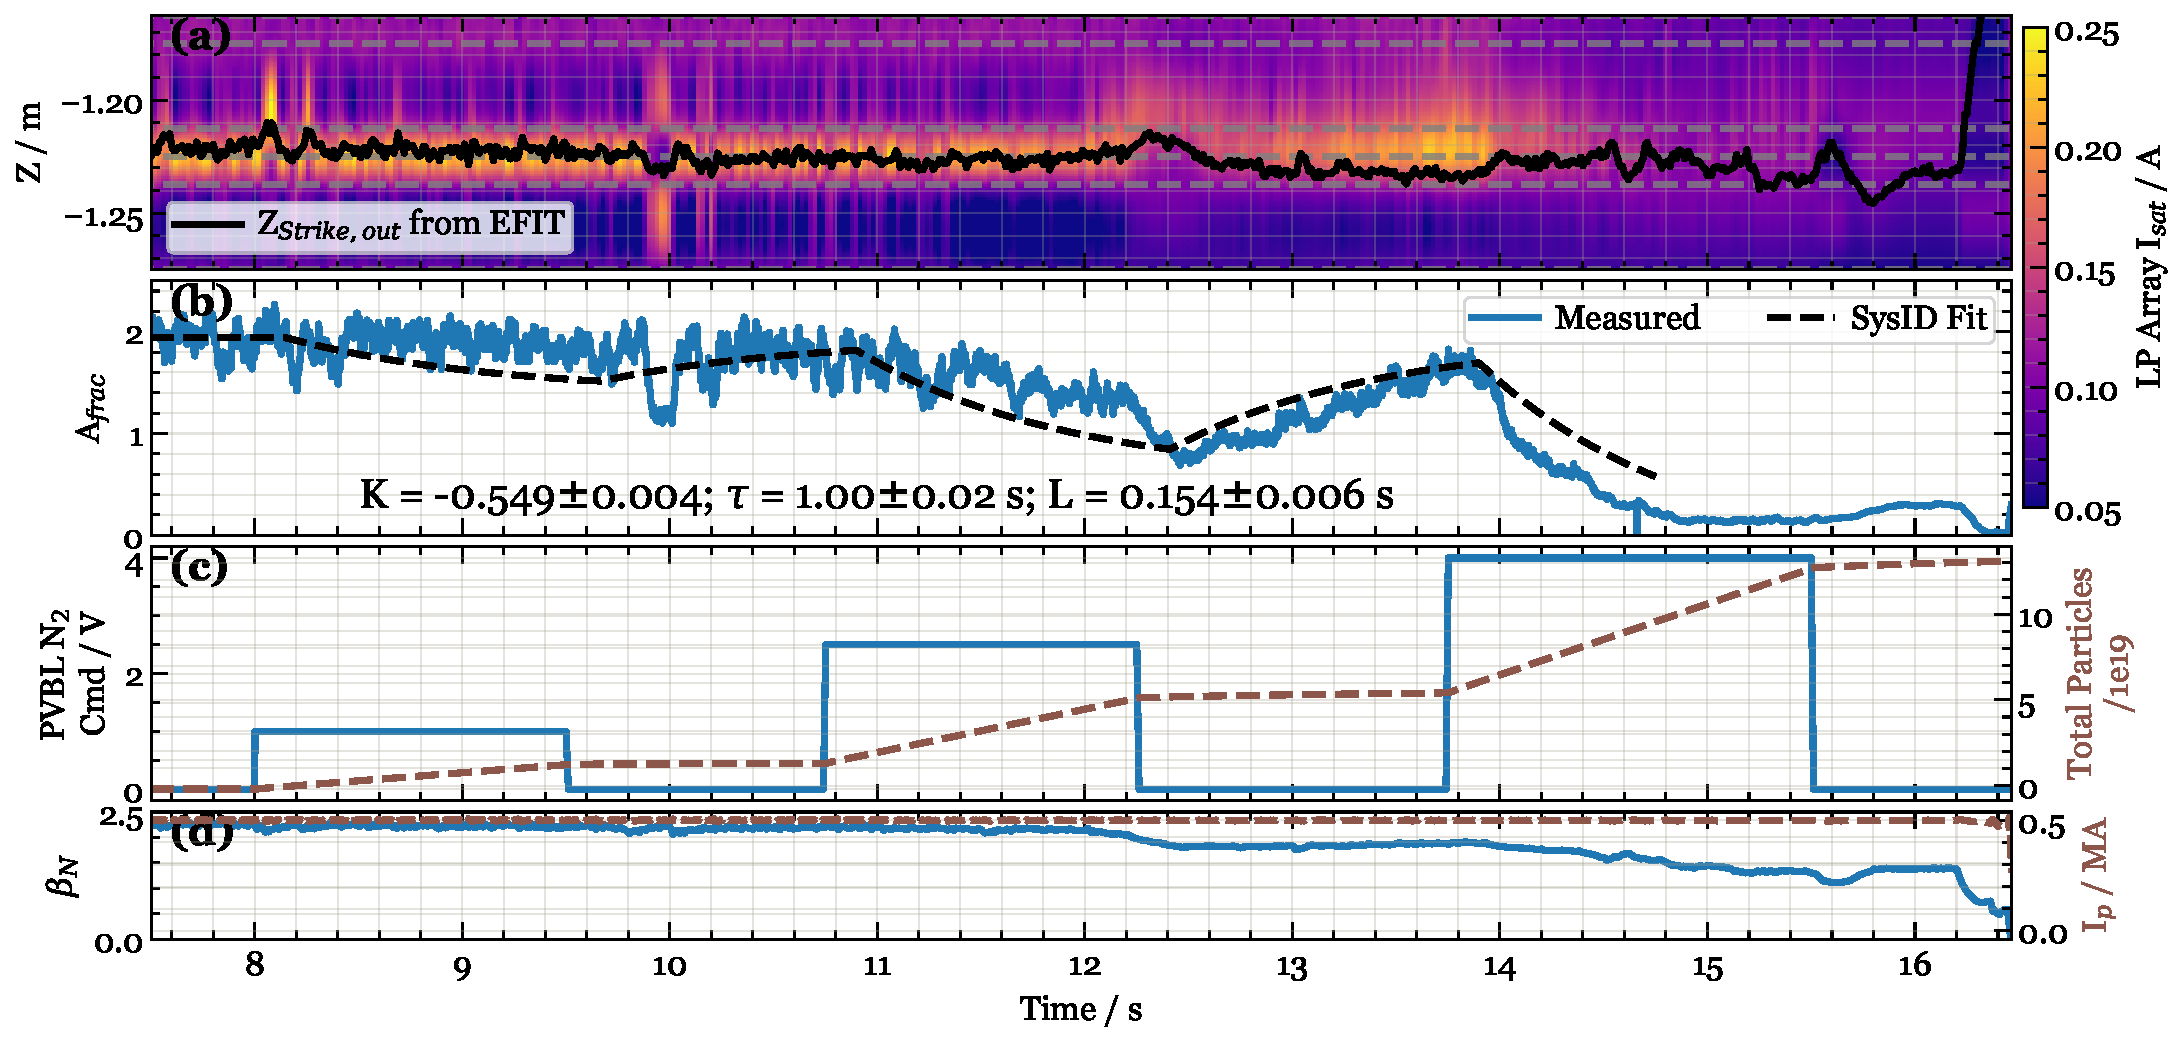
\includegraphics[width=\textwidth]{figures/DetCtrl_2D_35853.pdf}
 \caption{System identification shot \#35853.
(a) Shows the measured ion saturation current by realtime \ac{LP} array at locations marked by grey dashed lines.
The data has been interpolated spatially using cubic spline interpolation.
The black curve shows the post-shot calculated strike point position on outer divertor using EFIT.
(b) Shows the \Afrac calculated from peak value among the \ac{LP} array.
The dashed black line shows the system identification fit on this data.
(c) Left axis: Shows the N$_2$ gas command steps sent for system identification.
Right axis: Shows the cummulative N$_2$ gas particles injected into the vessel.
(d) Left axis: Shows $\beta_n$.
Right axis: Shows the plasma current (I$_p$).
$^*$ Note: \Afrac for this shot was not calibrated properly and the raw data reported 2 times the value.
We fixed this factor after this shot and this figure shows the corrected value.
}
 \label{fig:sysid_afrac}
\end{figure*}

\begin{figure}[!ht]
 \centering
 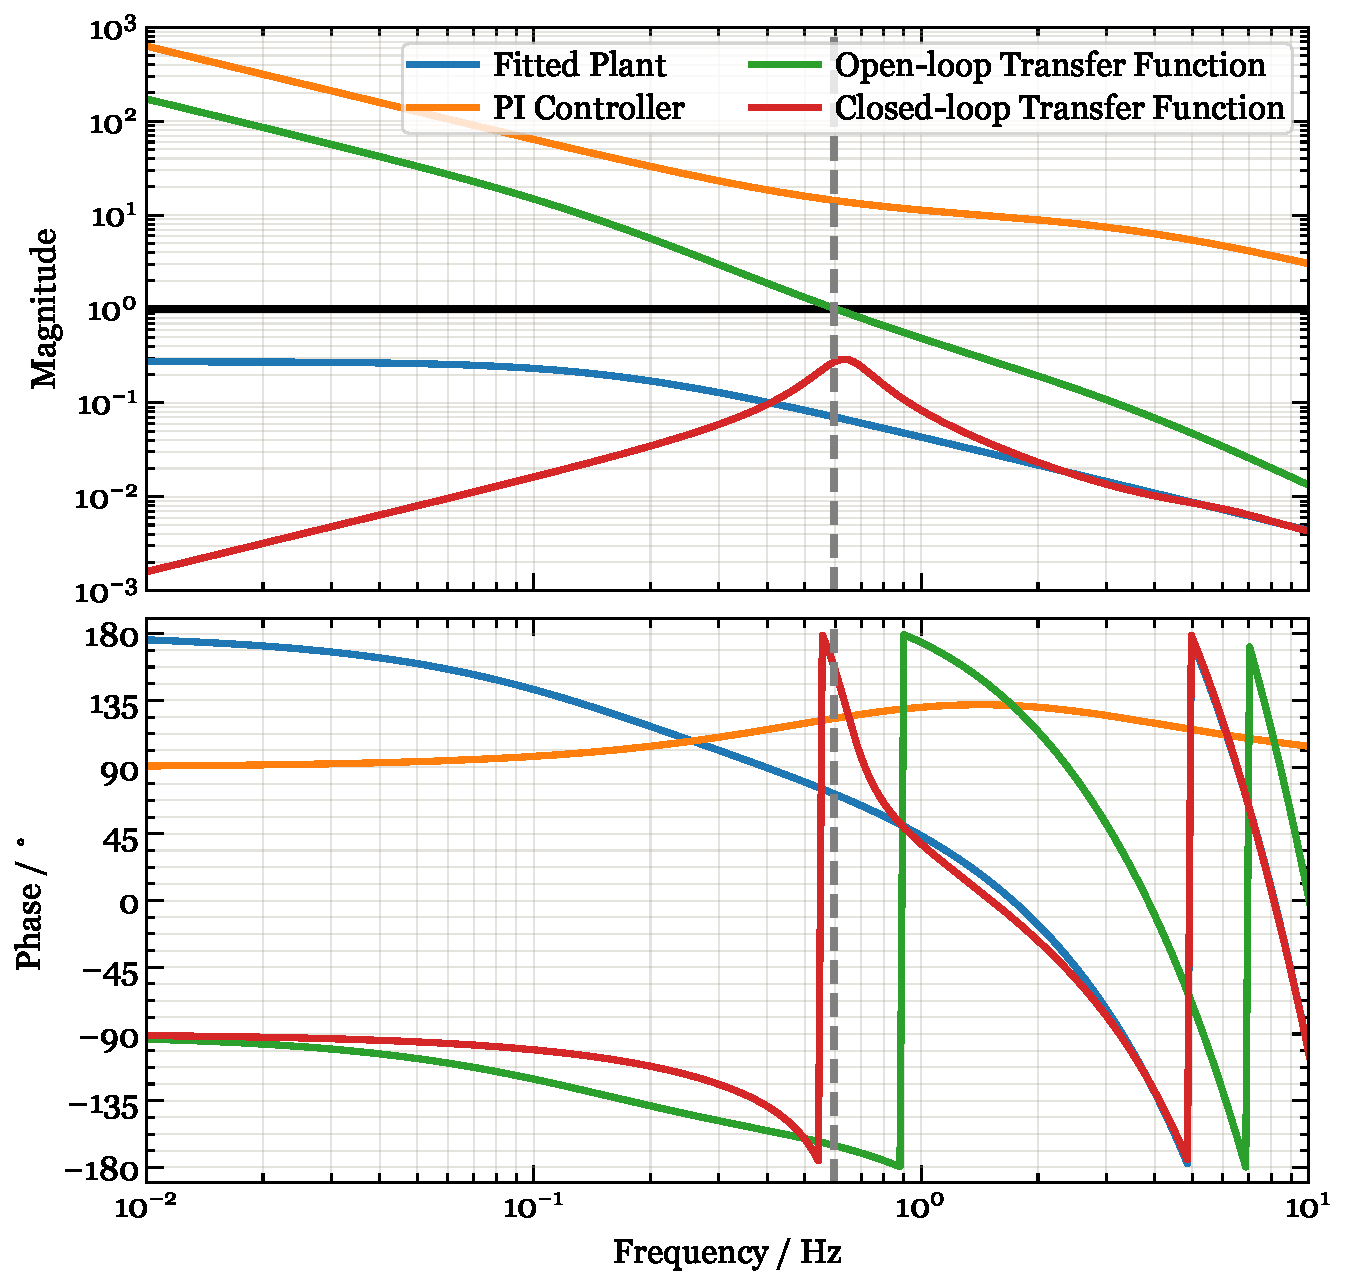
\includegraphics[width=\linewidth]{figures/Afrac_LoopStability.pdf}
 \caption{
Closed loop transfer function analysis of the system  using \Afrac output with chosen PI controller with gains:\AfracKp, \AfracTi, and \Afracstau.
The dashed grey verticle line shows the \ac{UGF} of the system.}
\label{fig:cltf_afrac}
\end{figure}

\section{System identification and Controller Tuning}
\label{sec:sysid}

\begin{figure*}[!ht]
 \centering
 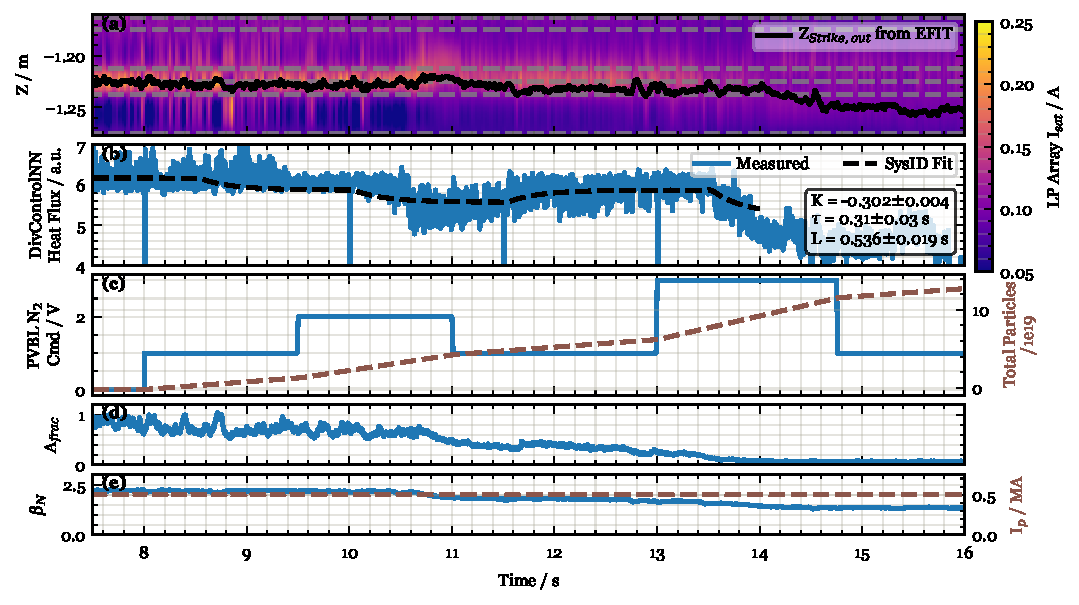
\includegraphics[width=\textwidth]{figures/DetCtrl_2D_35854.pdf}
 \caption{System identification shot \#35854.
(a) Shows the measured ion saturation current by realtime Langmuir Probe array at locations marked by grey dashed lines.
The data has been interpolated spatially using cubic spline interpolation.
The black curve shows the post-shot calculated strike point position on outer divertor using EFIT.
(b) Shows the heat flux at outer divertor calculated by DivControlNN.
The dashed black line shows the system identification fit on this data.
(c) Left axis: Shows the N$_2$ gas command steps sent for system identification.
Right axis: Shows the cummulative N$_2$ gas particles injected into the vessel.
(d) Shows the \Afrac calculated from peak value among the Langmuir probe array.
(e) Left axis: Shows $\beta_n$.
Right axis: Shows the plasma current (I$_p$).}
\label{fig:sysid_sm}
\end{figure*}

\begin{figure}[!ht]
 \centering
 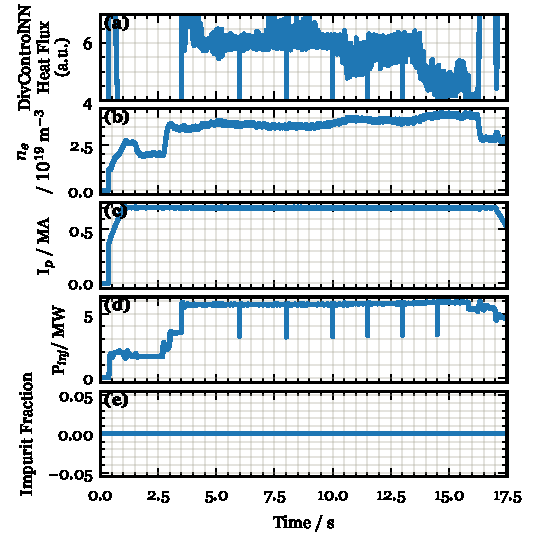
\includegraphics[width=\linewidth]{figures/SM_inputs_35854.pdf}
 \caption{
KSTAR \#35854 DivControlNN quantities.
(a) Shows the calculated heat flux at outer divertor calculated by DivControlNN.
Rest of the panels are inputs to DivControlNN.
(b) Shows the line averaged electron density.
(c) Shows the plasma current.
(d) Shows the total injected power.
(e) Shows the impurity fraction estimate.
Note that this calculation malfunctioned and fed constant zero input to the model even though N$_2$ was puffed in this shot.
Apart from these inputs, diffusion scaling factor was set to a constant value of 1.0 in the model.
}
 \label{fig:SM_inputs_35853}
\end{figure}

\begin{figure}[!h]
 \centering
 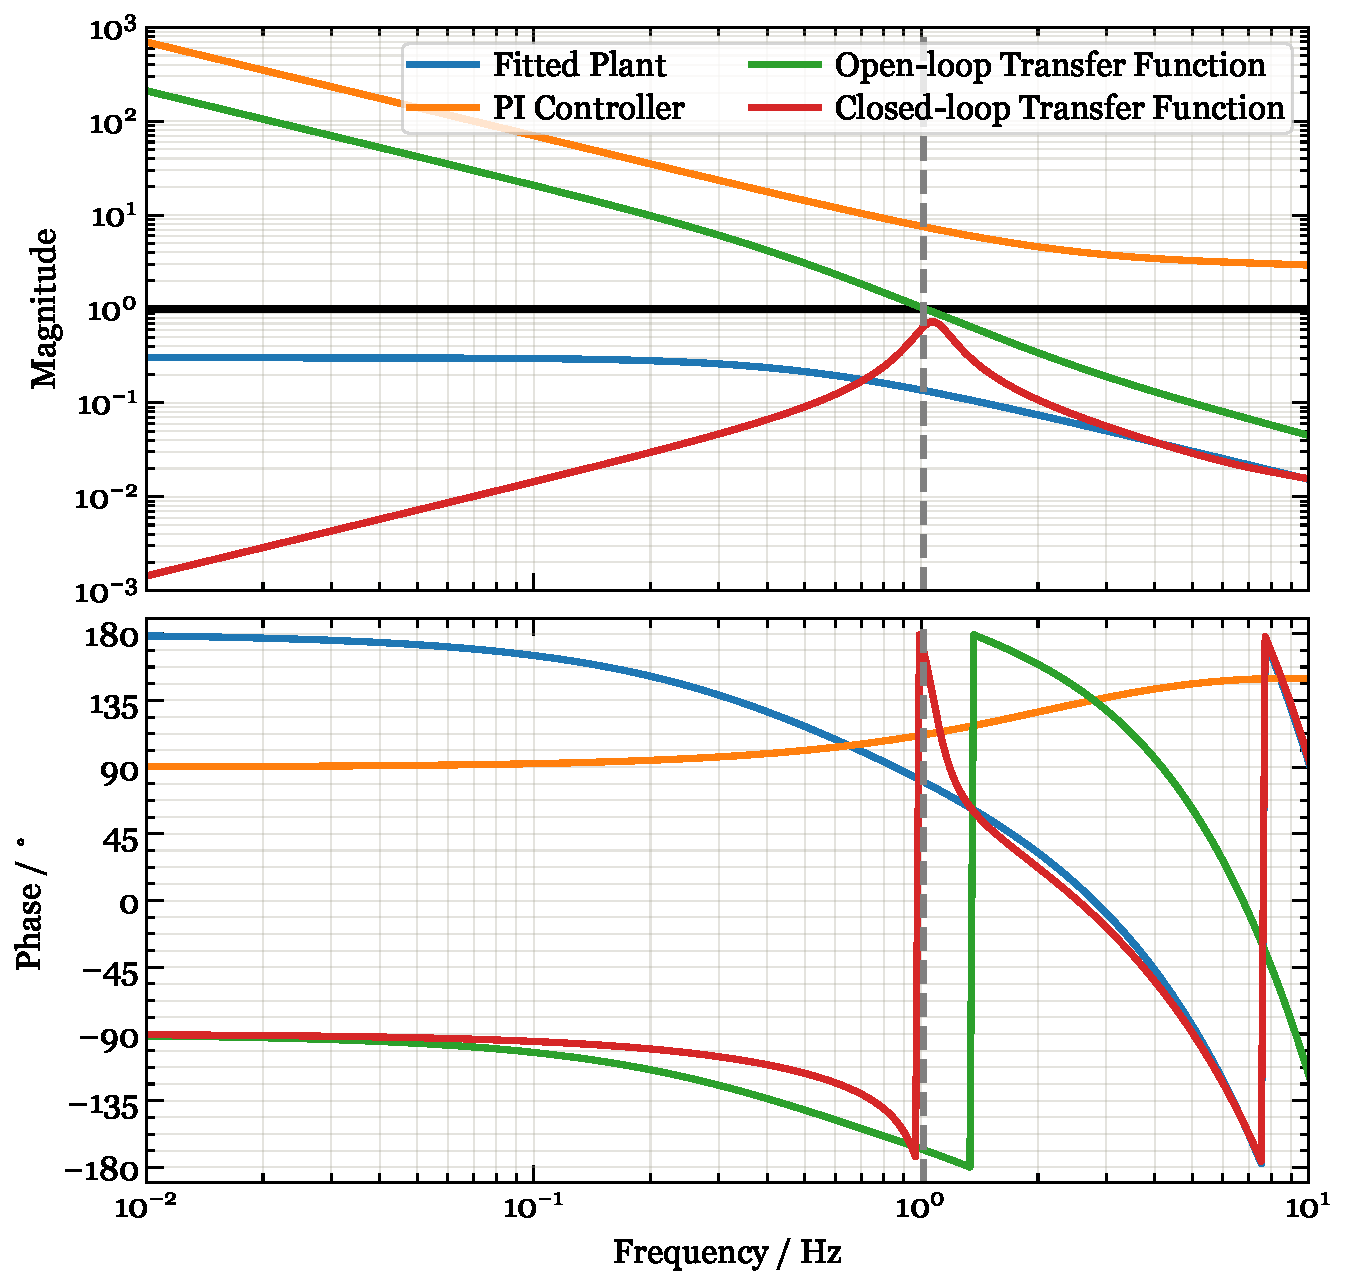
\includegraphics[width=\linewidth]{figures/SM_LoopStability.pdf}
 \caption{Closed loop transfer function analysis of the system using DivControlNN heat flux at outer divertor output with chosen PI controller with gains: \SMKp, \SMTi, and \SMstau.
The dashed grey verticle line shows the \ac{UGF} of the system.}
\label{fig:cltf_sm}
\end{figure}

Before we attempted detachment control experiments, we took two system identification shots.
The data from the first system identification shot \#35853 is shown in Fig.\ref{fig:sysid_afrac}.
In this shot, we puffed in N$_2$ gas in steps of 1.0 V, 2.5V, and 4.0 V with puff duration of 1.5s each.
A corresponding response was seen in \Afrac but with a delay.
We later confirmed from post-shot EFIT data that the strike point was indeed within the real-time Langmuir Probe array and thus our \Afrac calculation was valid.
We fitted the measured data with a simple first-order plant model (same as first order plus dead time\cite{Eldon_2022_PPCF}) of gain K, time constant $\tau$, and time delay $L$ given by (in Laplace domain):

\begin{equation}
 G(s) = \frac{K}{\tau s + 1}e^{-L s}
\label{eq:sysid}
\end{equation}

where $s$ is complex frequency variable in Laplace domain and $G(s)$ is the transfer function of the plant model.
The fit resulted in an identified model with \AfracK, \AfracTau, and \AfracL.
The fit is shown in Fig.\ref{fig:sysid_afrac}b.
Note that only the part of the time series data that was used in fit is shown for the fitted curve.
This fit was performed in the inter-shot interval during the experiment and has not been improved or modified after the experiment.

The controller gains were chosen by visualizing \ac{CLTF} of the system with chosen PI gains as shown in Fig.\ref{fig:cltf_afrac}.
Here, the frequency domain response of the plant model ($G(s)$) and PI controller ($T_{PI}(s)$) are plotted together.
When connected in series, this forms the \ac{OLTF} of the system ($O(s) = G(s) T_{PI}(s)$).
The frequency where \ac{OLTF} becomes 1.0 is called \ac{UGF}).
Phase margin is defined as the additional phase delay at \ac{UGF} that would make the system unstable by taking it to -180$^\circ$.
Additionally, we also define delay margin as the additional actuation delay that would make \ac{UGF} unstable.
The \ac{CLTF} is then calculated by solving the loop algebra in the Laplace domain:

\begin{equation}
 C(s) = \frac{G(s)}{1 + O(s)}
\label{eq:cltf}
\end{equation}

\begin{figure*}[!ht]
 \centering
 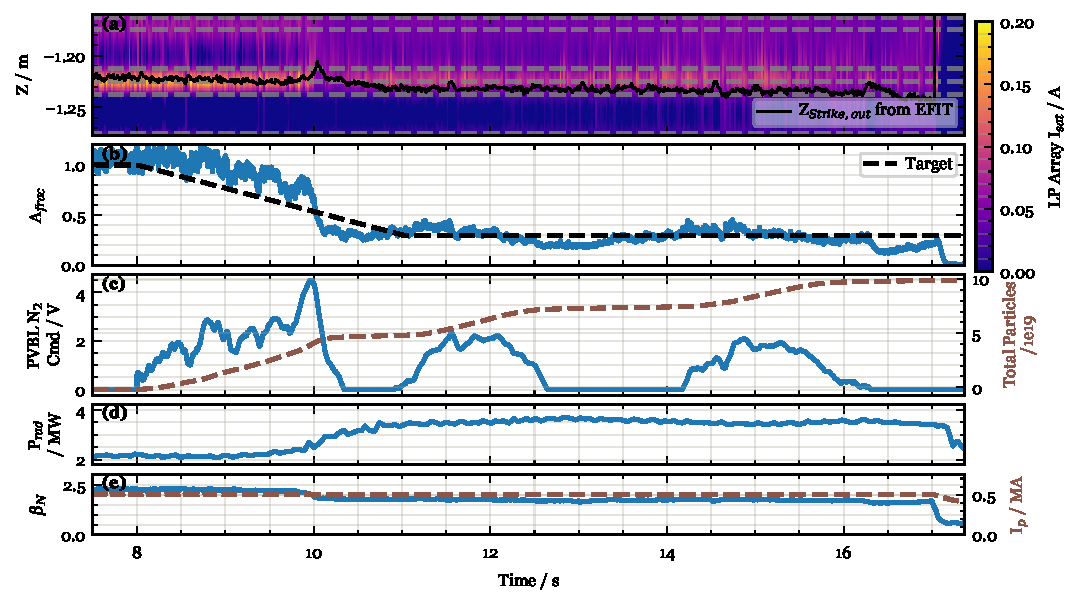
\includegraphics[width=\textwidth]{figures/DetCtrl_2D_35857.pdf}
 \caption{
Detachment control shot \# 35857 using \Afrac controller.
(a) Shows the measured ion saturation current by realtime Langmuir Probe array at locations marked by grey dashed lines.
The data has been interpolated spatially using cubic spline interpolation.
The black curve shows the post-shot calculated strike point position on outer divertor using EFIT.
(b) Shows the \Afrac calculated from peak value among the Langmuir probe array.
The dashed black line shows the target provided to the controller to follow.
(c) Left axis: Shows the N$_2$ gas command steps sent for system identification.
Right axis: Shows the cummulative N$_2$ gas particles injected into the vessel.
(d) Total radiated power measured by \ac{IRVB}.
(e) Left axis: Shows $\beta_n$.
Right axis: Shows the plasma current (I$_p$).
}
 \label{fig:detctrl_afrac}
\end{figure*}

Because of the long delay, we chose to not use a derivative gain.
The goal of tuning was to push \ac{UGF} as high as possible (\AfracUGF) while keeping a reasonable phase margin (\AfracPhaseMargin) and margin for any additional actuation delay (\AfracDelayMargin).
This resulted in controller settings as: \AfracKp, \AfracTi, and \Afracstau, where K$_p$ is proportional gain, T$_i$ is integral time, and $\tau_s$ is pre-smoothing time constant.
This is still a very aggressive choice of controller, but given that the system identification fit gave an unexpectedly high value of response time $\tau=1$s probably due to too much noise during small step inputs, we decided to go ahead with this controller choice.
The resulting PI controller transfer function is given by:

\begin{equation}
 T_{PI}(s) = K_p \left( \frac{1}{T_i s} + 1\right) \frac{1}{1 + \tau_s s}
\label{eq:PI}
\end{equation}

Unfortunately, the surrogate model was not configured properly in this system identification shot due to technical errors, so we repeated a system identification but this time we decided to keep the nitrogen valve in the constant open position, to look for any deviation in the behavior.
The data from this second system identification shot is shown in Fig.\ref{fig:sysid_sm}.
Despite all the limitations of DivControlNN as listed earlier, we still saw a good correlation in the DivControlNN heat flux output at the outer divertor with the injected gas as seen in Fig.\ref{fig:sysid_sm}b.
This is validated by estimated \Afrac in Fig.\ref{fig:sysid_sm}d showing an increase in detachment level as the predicted output heat flux decreases.
The strike point was maintained within the realtime Langmuir probe array (Fig.\ref{fig:sysid_sm}a) validating the output of \Afrac.
Note that we have not yet calibrated the DivControlNN model with any experimental data, so we treated the output as arbitrary units and later attempted to control the detachment with estimated changes to this arbitrary output.

Fig.\ref{fig:SM_inputs_35854} shows the time-varying inputs to DivControlNN along with the heatflux output from the model.
Here, note that the impurity fraction input to the model malfunctioned, and a constant zero impurity fraction was fed to the model even though we puffed in N$_2$ in this system identification test. During the test part from 7.5~s onwards, we can see that most inputs to the model remained mostly constant, and only the line-averaged electron density showed considerable changes.
It can be seen thus that at this time, DivControlNN solely relied on changes in the electron density to estimate heat flux at the outer divertor.
The malfunctioning of the impurity fraction was detected in the post-processing of the data, and thus, during the experiment, we continued to try to use this model as it was.

We again fitted this system with a first-order system with a delay as described in Eq.\ref{eq:sysid}.
The fit resulted in an identified model with \SMK, \SMTau, and \SML.
The fit is shown in Fig.\ref{fig:sysid_sm}b.
Here as well, the fitting shown was performed during the experiment in the inter-shot interval and has not been modified or optimized later.
The time domain in which the fitting curve is shown is the data where the system was fitted.
Admittedly, this fit was not very good and we did not believe the large lag value to be accurate.
So for the purpose of tuning the controller, we arbitrarily set the system lag value to 100 ms.
The controller gains were chosen by visualizing \ac{CLTF} of the system with chosen PI gains as shown in Fig.\ref{fig:cltf_sm} and following the same procedure as we described for \Afrac controller tuning.
The resulting controller settings were: \SMKp, \SMTi, and \SMstau{} creating controller given by Eq.\ref{eq:PI}.
Here, we estimated to achieve a \ac{UGF} of \SMUGF, phase margin of \SMPhaseMargin, and delay margin of \SMDelayMargin.
This controller was also very aggressive, but we decided to go ahead with this controller choice given the limitations of the system identification fit and lack of time for further analysis in between the allotted run time of our experiment.
We understand that the system identification procedure is fitting a more complex and probably non-linear model with a simple linear model, and thus the above mentioned controller tuning technique is at best a good way to come up with an intial controller that can be adjusted better after the first closed loop test
